\documentclass{article}
\usepackage[margin=2cm]{geometry}
\usepackage[utf8]{inputenc}
\usepackage{minted}

\title{CSC258 PRELAB 5}
\author{Tingfeng Xia}
\date{October 2019}

\usepackage{natbib}
\usepackage{graphicx}

\begin{document}

\maketitle
\section*{PART 1}
\paragraph{(1) \& (2)} Here is my schematic
\begin{center}
	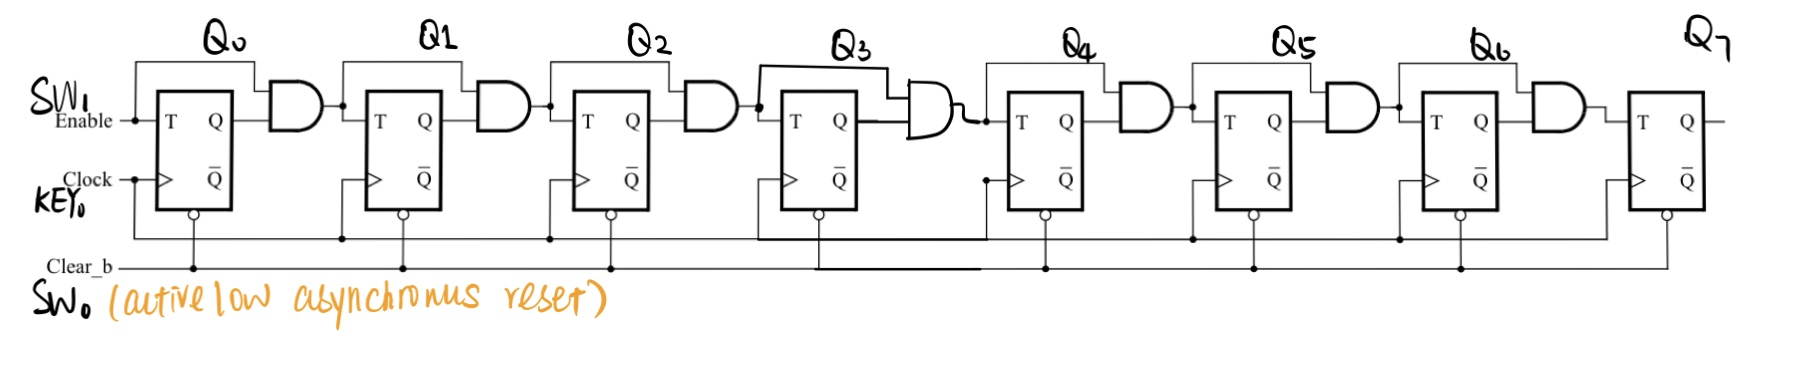
\includegraphics[scale=0.25]{q1_scheme.jpg}
\end{center}
\paragraph{(3)} Here is my verlog code for the 8 bit counter as drawn above:
\begin{minted}{verilog}
    module CounterSynchronus(SW, KEY, HEX0, HEX1);
    	// main module
    	input [1:0]SW;
    	input [0:0] KEY;
    	output [6:0] HEX0;
    	output [6:0] HEX1;
    	
    	wire [7:0] twohex;
    	
    	counter8(
    		.enable(SW[1]), 	// if incre
    		.clk(KEY[0]),  	// clock signal
    		.clear_b(SW[0]), 	// reset
    		.Q(twohex)
    	);
    	
    	// lower four bits
    	hex hex0(twohex[3:0], HEX0);
    	// upper four bits
    	hex hex1(twohex[7:4], HEX1);
    	
    endmodule
    
    module counter8(enable, clk, clear_b, Q);
    	input enable, clk, clear_b;
    	output [7:0] Q;
    	
    	// seven 'and' parts of the circuit
    	wire w0, w1, w2, w3, w4, w5, w6;
    	assign w0 = (enable & Q[0]);
    	assign w1 = (w0 & Q[1]);
    	assign w2 = (w1 & Q[2]);
    	assign w3 = (w2 & Q[3]);
    	assign w4 = (w3 & Q[4]);
    	assign w5 = (w4 & Q[5]);
    	assign w6 = (w5 & Q[6]);
    	
    	// Connecting the flip flops
    	TFlipFlop t0(enable, clk, clear_b, Q[0]);
    	TFlipFlop t1(w0, clk, clear_b, Q[1]);
    	TFlipFlop t2(w1, clk, clear_b, Q[2]);
    	TFlipFlop t3(w2, clk, clear_b, Q[3]);
    	TFlipFlop t4(w3, clk, clear_b, Q[4]);
    	TFlipFlop t5(w4, clk, clear_b, Q[5]);
    	TFlipFlop t6(w5, clk, clear_b, Q[6]);
    	TFlipFlop t7(w6, clk, clear_b, Q[7]);
    	
    endmodule	
    
    // Not to name this t_f_f
    module TFlipFlop(T, clk, clear_b, Q);
    	input T;
    	input clk;
    	input clear_b;
    	output reg Q;
    	always @(posedge clk, negedge clear_b)
    	begin
    		if (clear_b == 1'b0)
    			Q <= 1'b0;
    		else if (clear_b == 1'b1)
    			Q <= ~Q;
    	end
    endmodule
    
    // Rewritten shorter version of hexdecoder
    // The previes version was too cumbersome
    // 	to include in pdf reports
    module hex(in, out);
    	input [3:0] in;
    	output [6:0] out;
    	reg [6:0] z;
    	always @(*)
    	begin
    		case (in[3:0])
    			4'b0000: z = 7'b1111110;
    			4'b0001: z = 7'b0110000;
    			4'b0010: z = 7'b1101101; 
    			4'b0011: z = 7'b1111001;
    			4'b0100: z = 7'b0110011;
    			4'b0101: z = 7'b1011011;  
    			4'b0110: z = 7'b1011111;
    			4'b0111: z = 7'b1110000;
    			4'b1000: z = 7'b1111111;
    			4'b1001: z = 7'b1111011;
    			4'b1010: z = 7'b1110111; 
    			4'b1011: z = 7'b0011111;
    			4'b1100: z = 7'b1001110;
    			4'b1101: z = 7'b0111101;
    			4'b1110: z = 7'b1001111;
    			4'b1111: z = 7'b1000111;
    		endcase
    	end
    	assign out[6:0] = z[6:0];
    endmodule 
\end{minted}
% \paragraph{(4)} Simulation of the module

\paragraph{(4) (5)} Simulation for the augmented module.
\begin{center}
    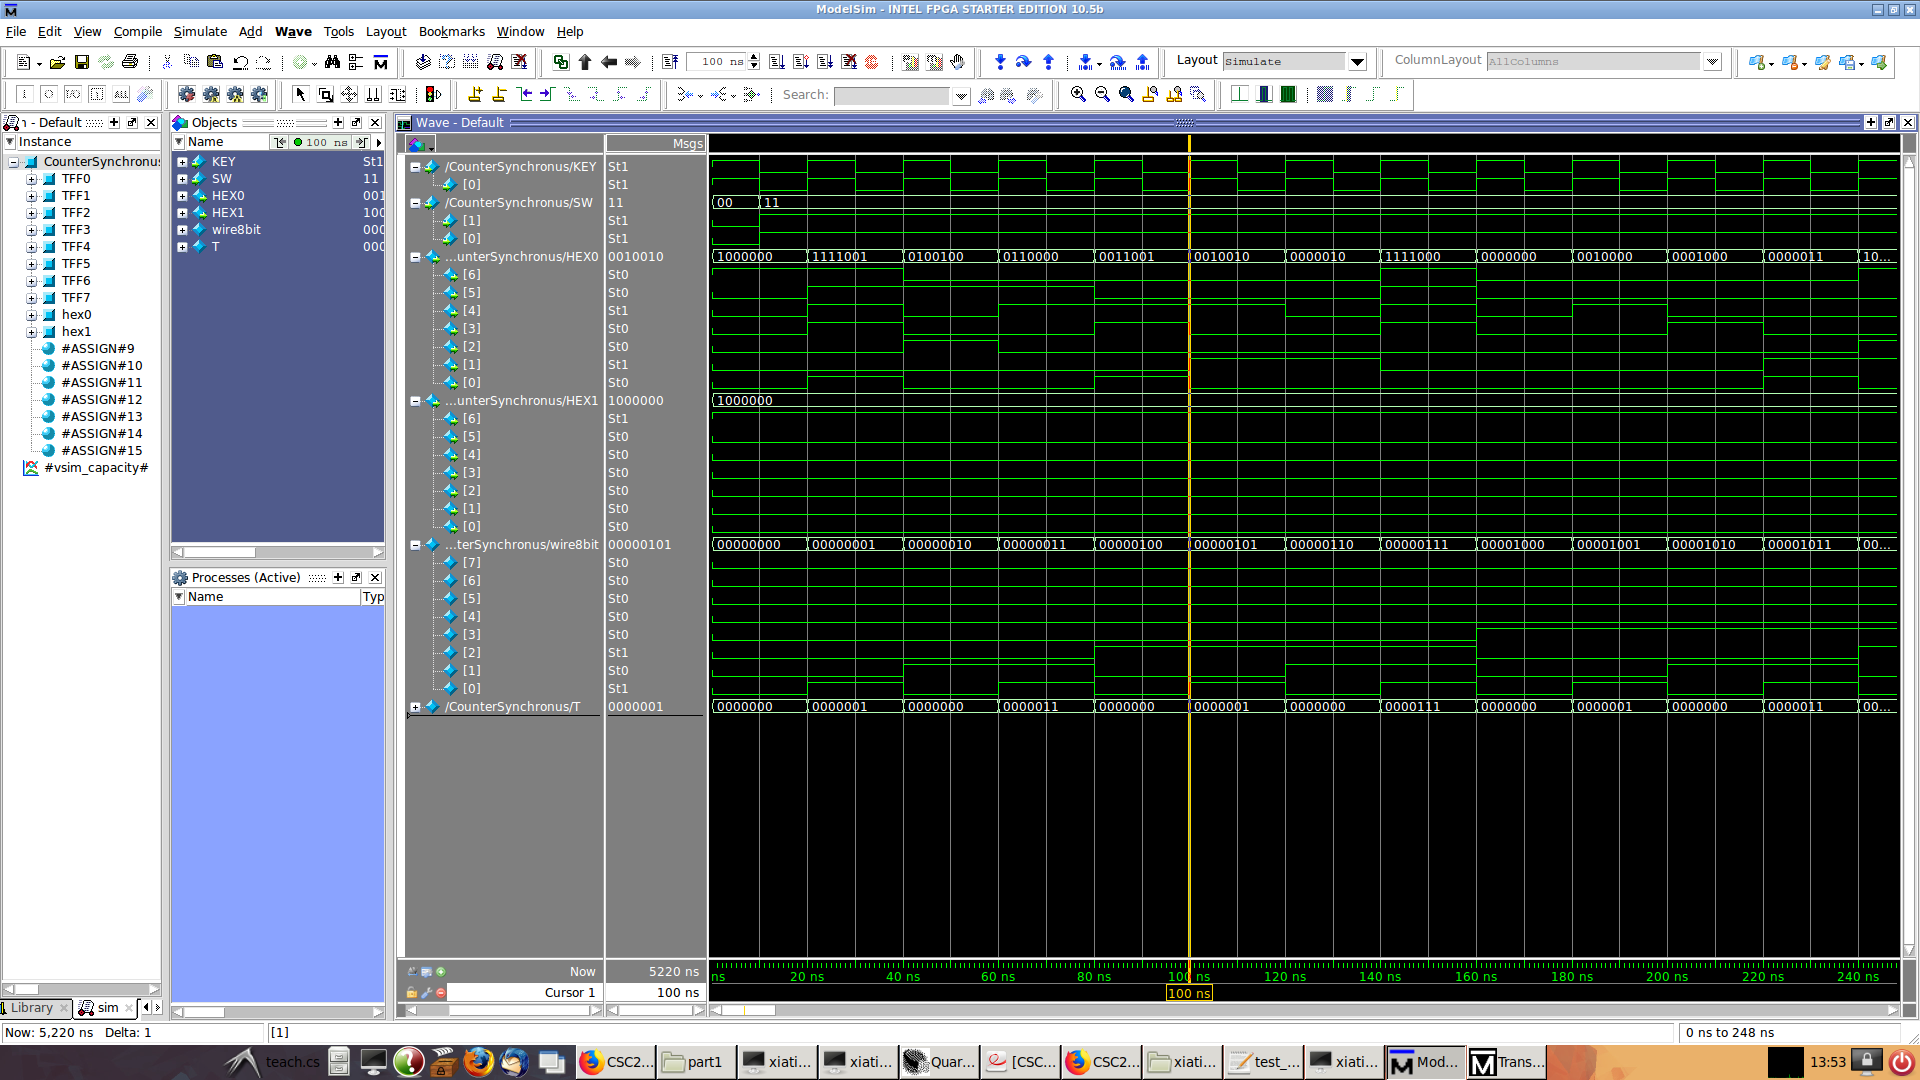
\includegraphics[scale=0.25]{q1_model_sim.png}
\end{center}{}
\paragraph{(6a)} Here is the screen shot for the ALM logic utilization report
\begin{center}
    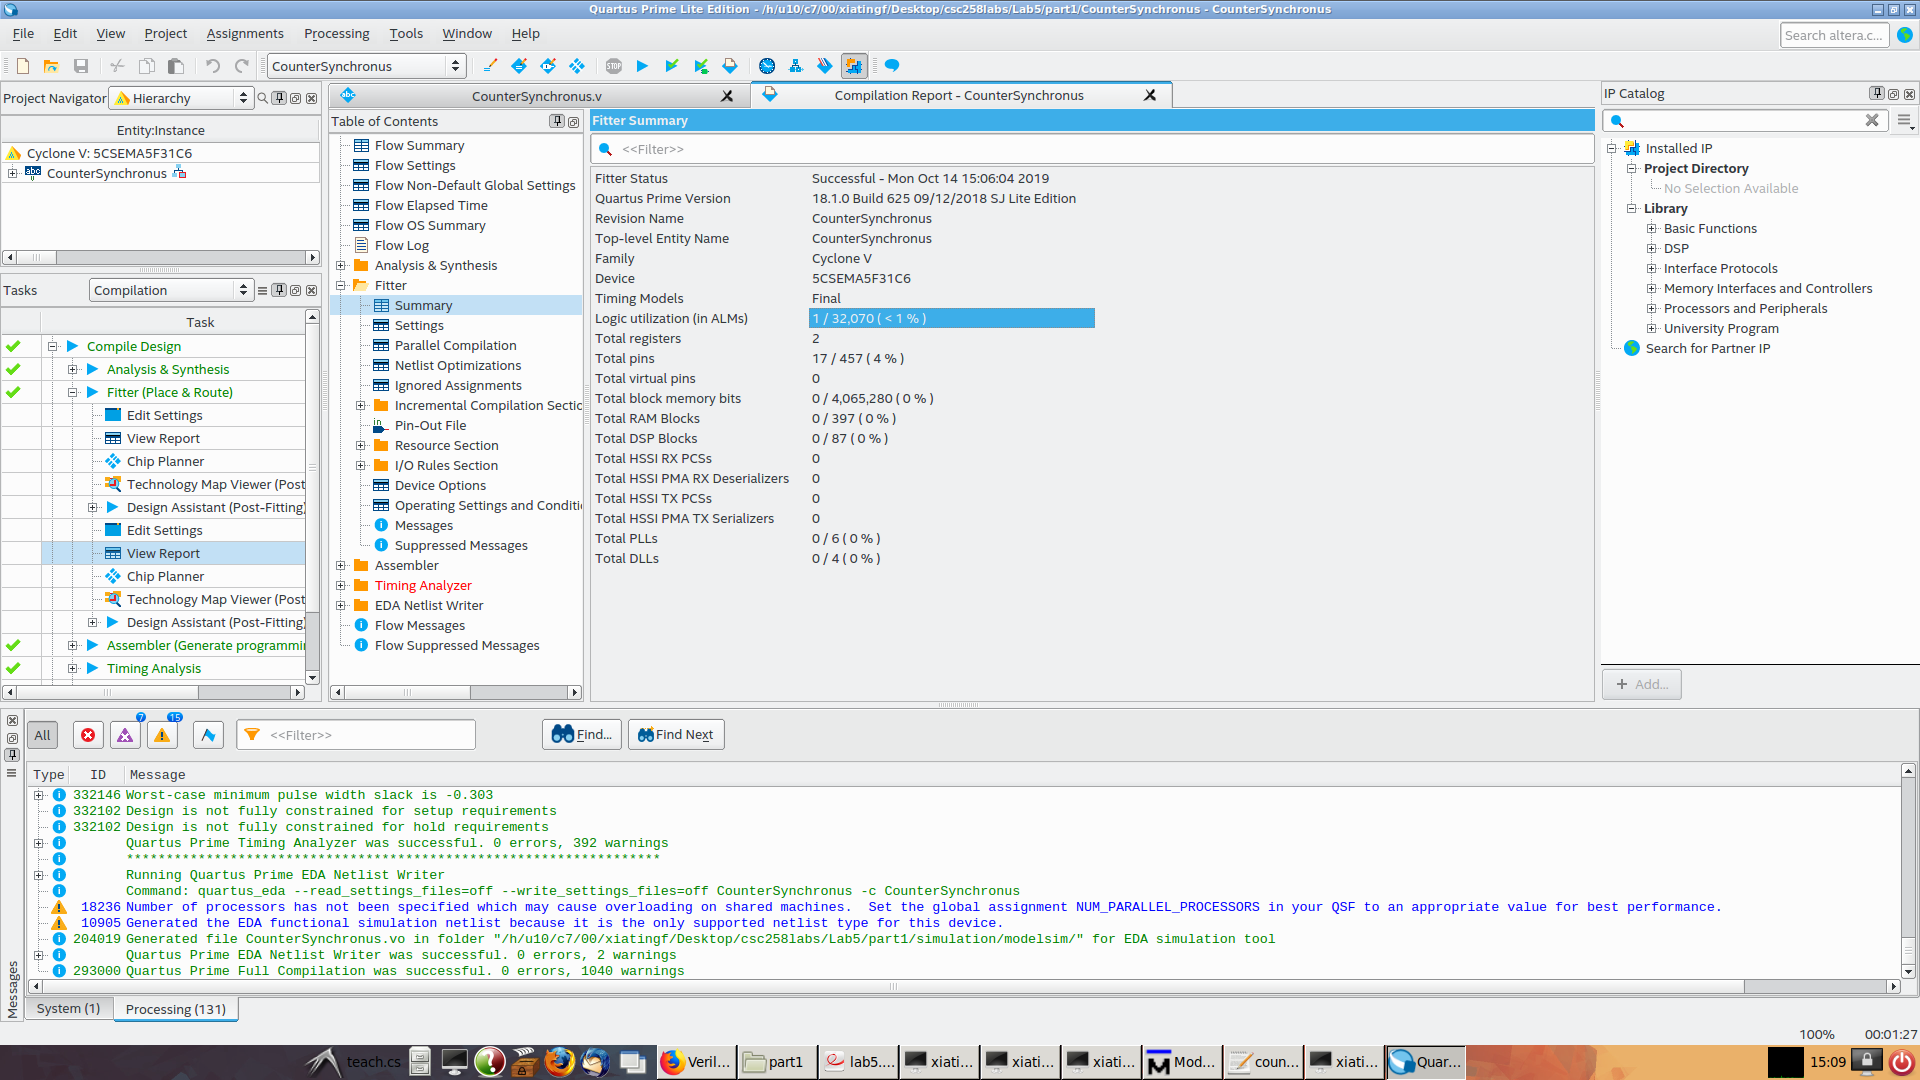
\includegraphics[scale=0.25]{q1_6a.png}
\end{center}

\paragraph{(6b)} 
\begin{center}
    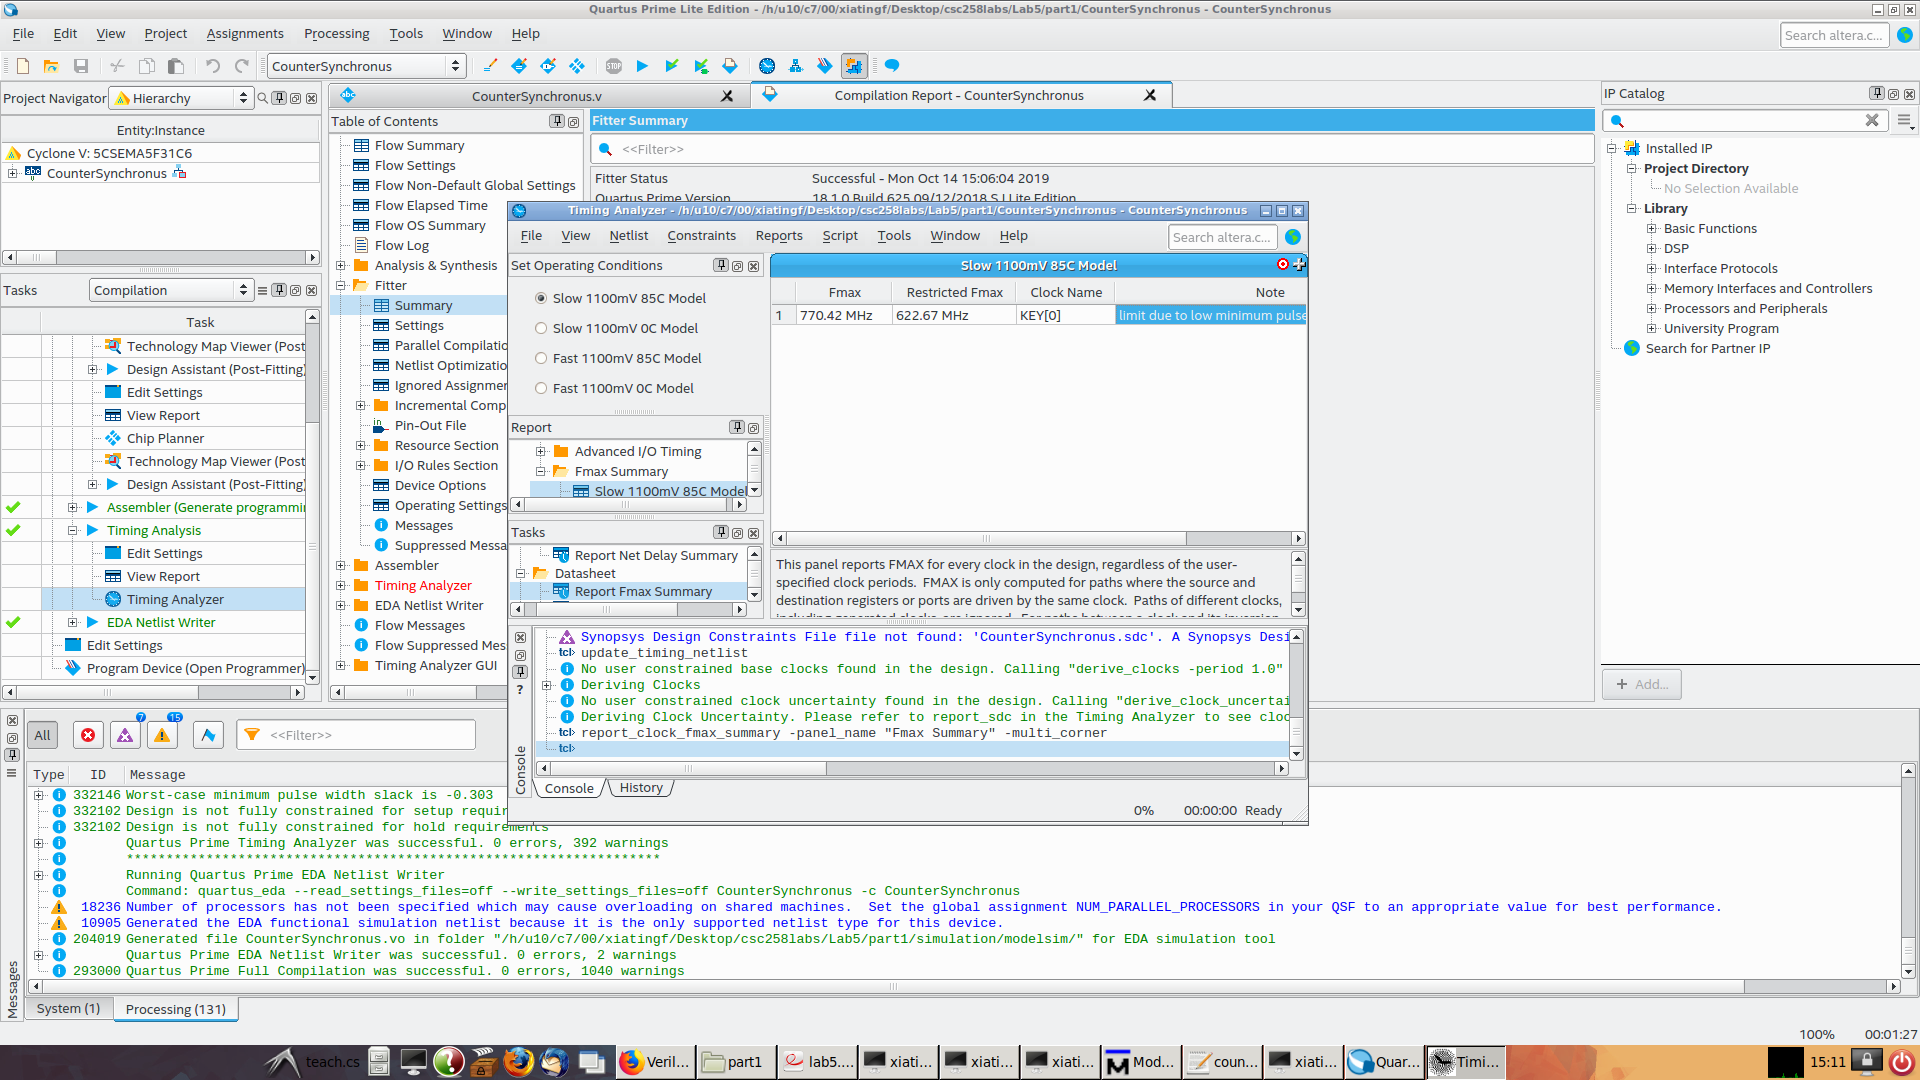
\includegraphics[scale=0.25]{q1_6b.png}
\end{center}

\paragraph{(7)} Quartus Prime Implementation
\begin{center}
    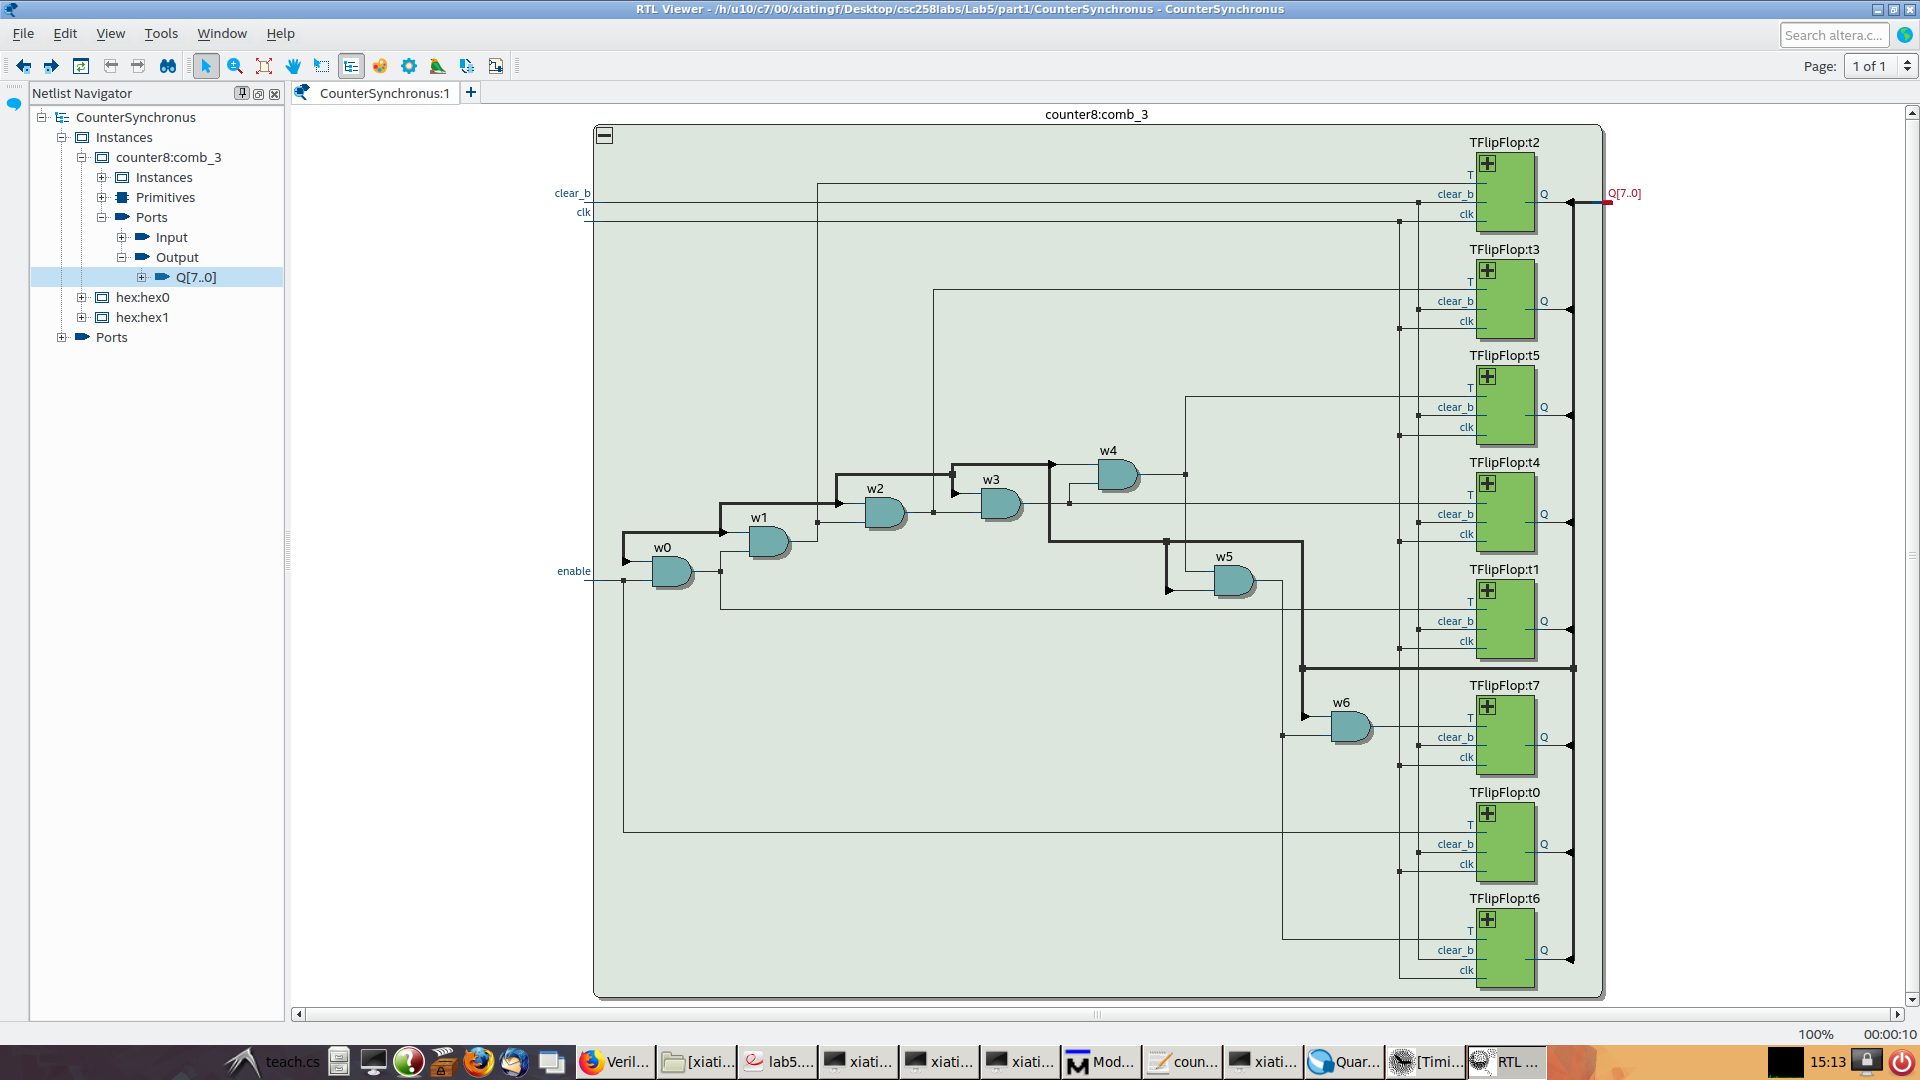
\includegraphics[scale=0.25]{q1_7.png}
\end{center}

\section*{PART 2}
\begin{itemize}
    \item Thanks to the limit in the number of digits, I don't need to check the maximum value
    \item I need two four bit counters. When the first counter reaches 1111, send a 1 to the enable to the next counter. Monitor the total result (9 in binary is 00001\_0001)
    \item I will see all numbers, but since it is flashing tooooo fast, I will just see an 8.
    \item 50Mega 
    \item requires 26 bits to represent (here since counters are of 4 bits, we need 7 of them; total of 28 bits)
\end{itemize}

\paragraph{(1)} Sorry I missed this part initially since I have coded my circuit, I will let quartus do this job for me. 
\begin{center}
    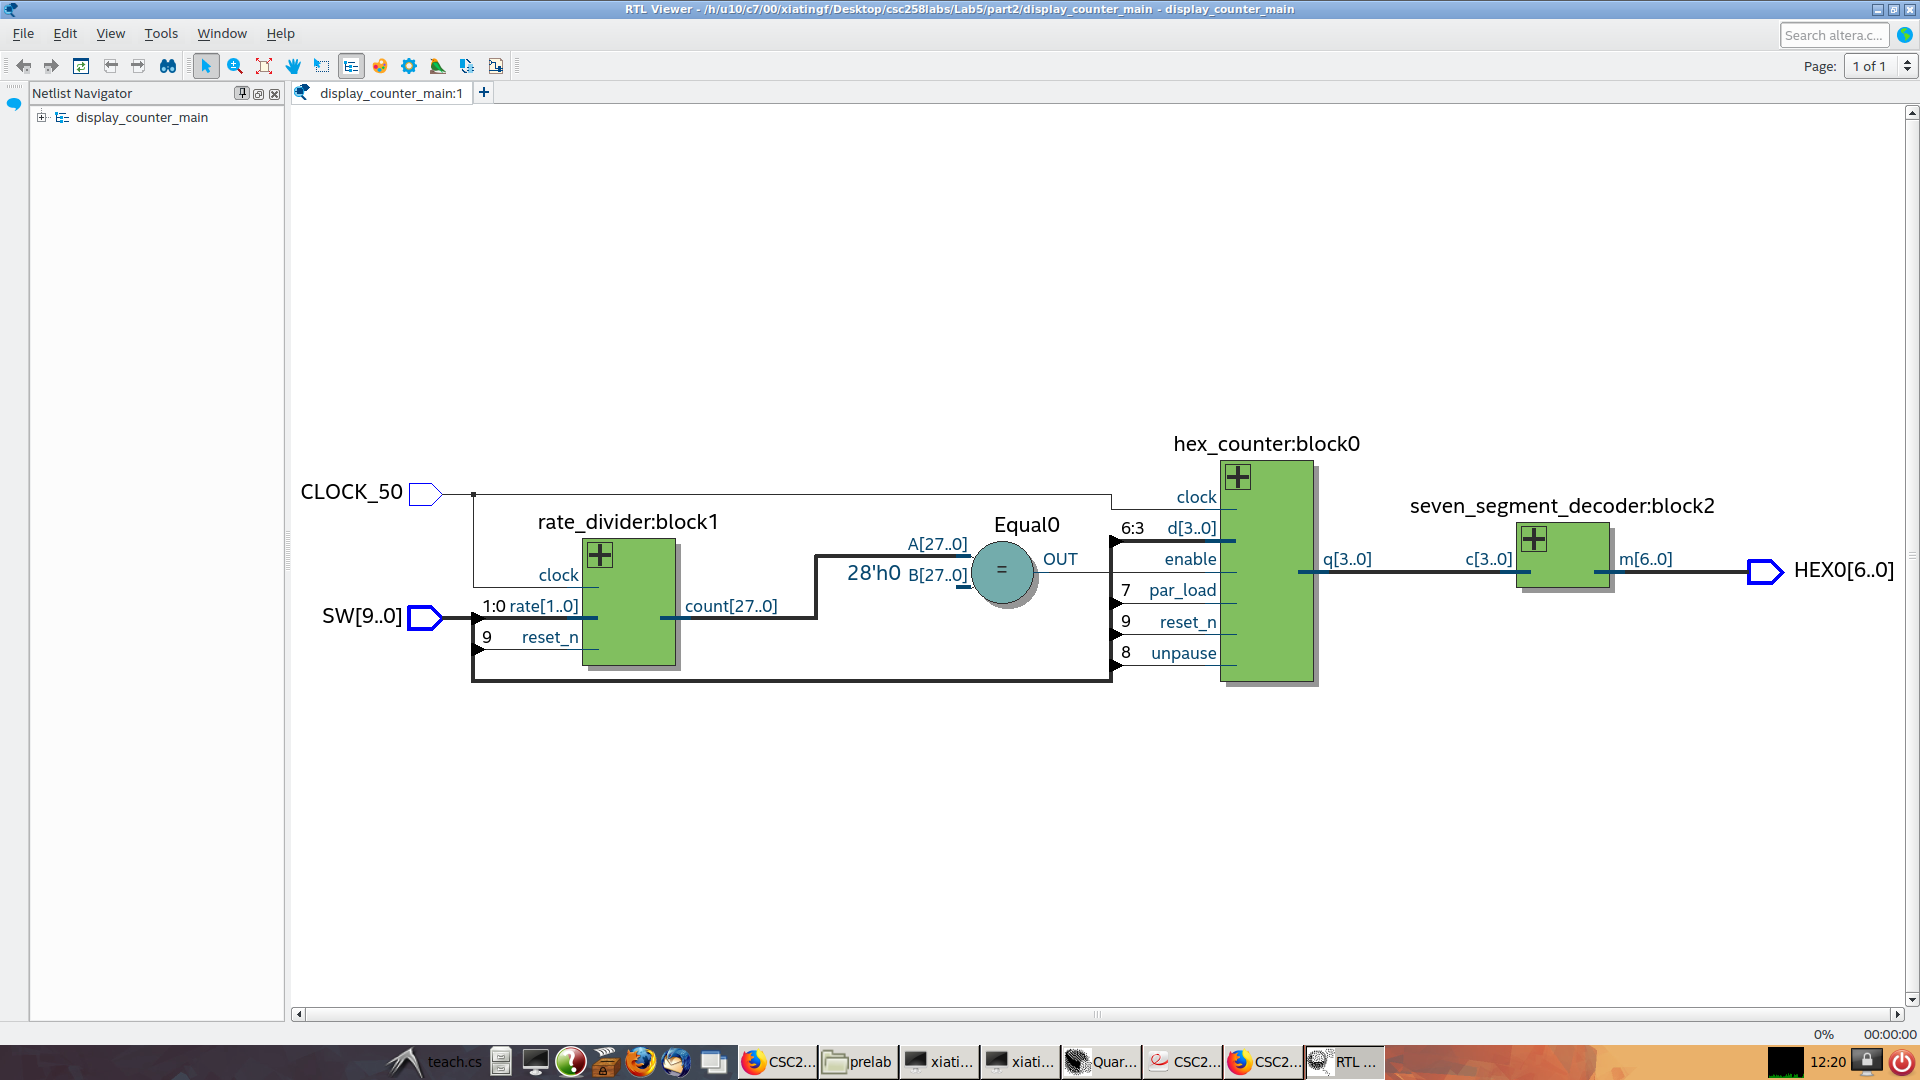
\includegraphics[scale=0.25]{part2_q1.png}
\end{center}
\paragraph{(2)} Here is my verilog code for the rate divider
\begin{minted}{verilog}
    module display_counter_main(SW, HEX0, CLOCK_50);
    	input [9:0] SW;
    	input CLOCK_50;
    	
    	output [6:0] HEX0;
    	
    	wire enable;
    	wire [27:0] RateDivider;
    	assign enable = (RateDivider == 28'd0) ? 1 : 0;
    	
    	wire [3:0] Q;
    	
    	hex_counter block0(
    		.d(SW[6:3]), //Load value
    		.clock(CLOCK_50),
    		.reset_n(SW[9]),
    		.par_load(SW[7]),
    		.enable(enable),
    		.unpause(SW[8]),
    		.q(Q)
    	);
    	
    	rate_divider block1(
    		.rate(SW[1:0]),
    		.clock(CLOCK_50),
    		.reset_n(SW[9]),
    		.count(RateDivider)
    	);
    	
    	hex block2(
    		.c(Q[3:0]),
    		.m(HEX0[6:0])
    	);
    endmodule
    	
    
    
    // hex_counter's enable is determined by clock divider.
    module hex_counter(d, clock, reset_n, par_load, enable, q, unpause);
    	input [3:0] d;
    	input clock;
    	input reset_n;
    	input unpause;
    	input par_load, enable;
    	output [3:0] q;
    	reg [3:0] q;
    	
    	
    	
    	always @(posedge clock, negedge reset_n, posedge par_load)
    	begin
    		if (reset_n == 1'b0)
    			q <= 0;
    		else if (par_load == 1'b1)
    			q <= d;
    		else if (enable == 1'b1 & unpause == 1'b1)
    			begin
    				if (q == 4'b1111)
    					q <= 0;
    				else 
    					q <= q + 1'b1;
    			end
    	end
    
    endmodule
    	
    module rate_divider(rate, clock, reset_n, count);
    	input [1:0] rate;
    	input reset_n;
    	input clock;
    	output [27:0] count;
    	reg [27:0] count;
    	reg [27:0] scale;
    	always @(*)
    	begin
    	     case (rate[1:0])
    		      2'b00: scale = 0;
    				2'b01: scale = 1;
    				2'b10: scale = 2;
    				2'b11: scale = 4;
    		  endcase
    	end
    	 
    
    	always @(posedge clock)
    		if (rate[1:0] != 2'b00)
    		begin 
    			 if (reset_n == 1'b0)
    				  count <= 5 * (10 ** 7) * scale - 1;
    			 else if (count == 0)
    				  count <= 5 * (10 ** 7) * scale - 1;
    			 else
    				  count <= count - 1;
    		end
    		else
    		    count <= 0;
    
    endmodule
    
    // Rewritten shorter version of hexdecoder
    // The previes version was too cumbersome
    // 	to include in pdf reports
    module hex(c, m);
    	input [3:0] c;
    	output [6:0] m;
    	reg [6:0] z;
    	always @(*)
    	begin
    		case (c[3:0])
    			4'b0000: z = 7'b1111110;
    			4'b0001: z = 7'b0110000;
    			4'b0010: z = 7'b1101101; 
    			4'b0011: z = 7'b1111001;
    			4'b0100: z = 7'b0110011;
    			4'b0101: z = 7'b1011011;  
    			4'b0110: z = 7'b1011111;
    			4'b0111: z = 7'b1110000;
    			4'b1000: z = 7'b1111111;
    			4'b1001: z = 7'b1111011;
    			4'b1010: z = 7'b1110111; 
    			4'b1011: z = 7'b0011111;
    			4'b1100: z = 7'b1001110;
    			4'b1101: z = 7'b0111101;
    			4'b1110: z = 7'b1001111;
    			4'b1111: z = 7'b1000111;
    		endcase
    	end
    	assign m[6:0] = z[6:0];
    endmodule 
\end{minted}
\paragraph{(3)} Here is my simulation for the rate divider module
\begin{center}
    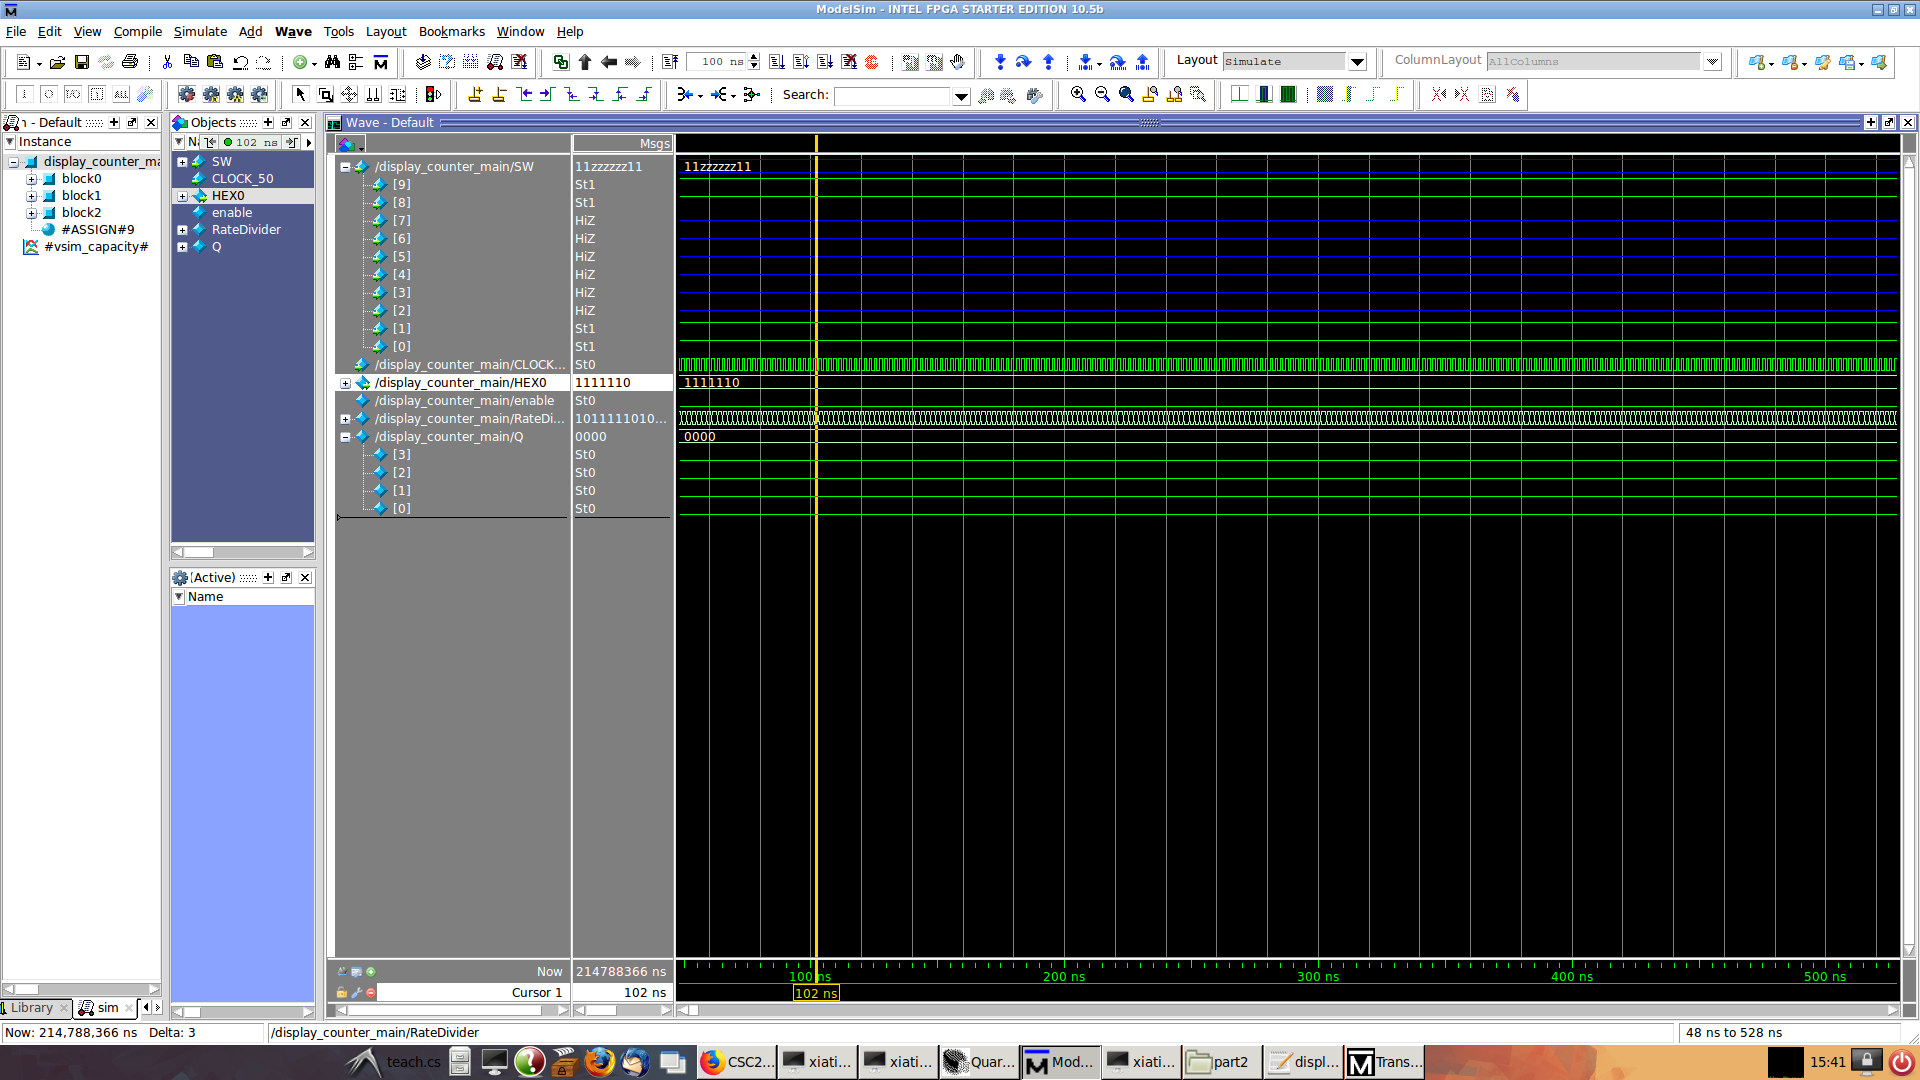
\includegraphics[scale=0.25]{q2_full_freq.png}
    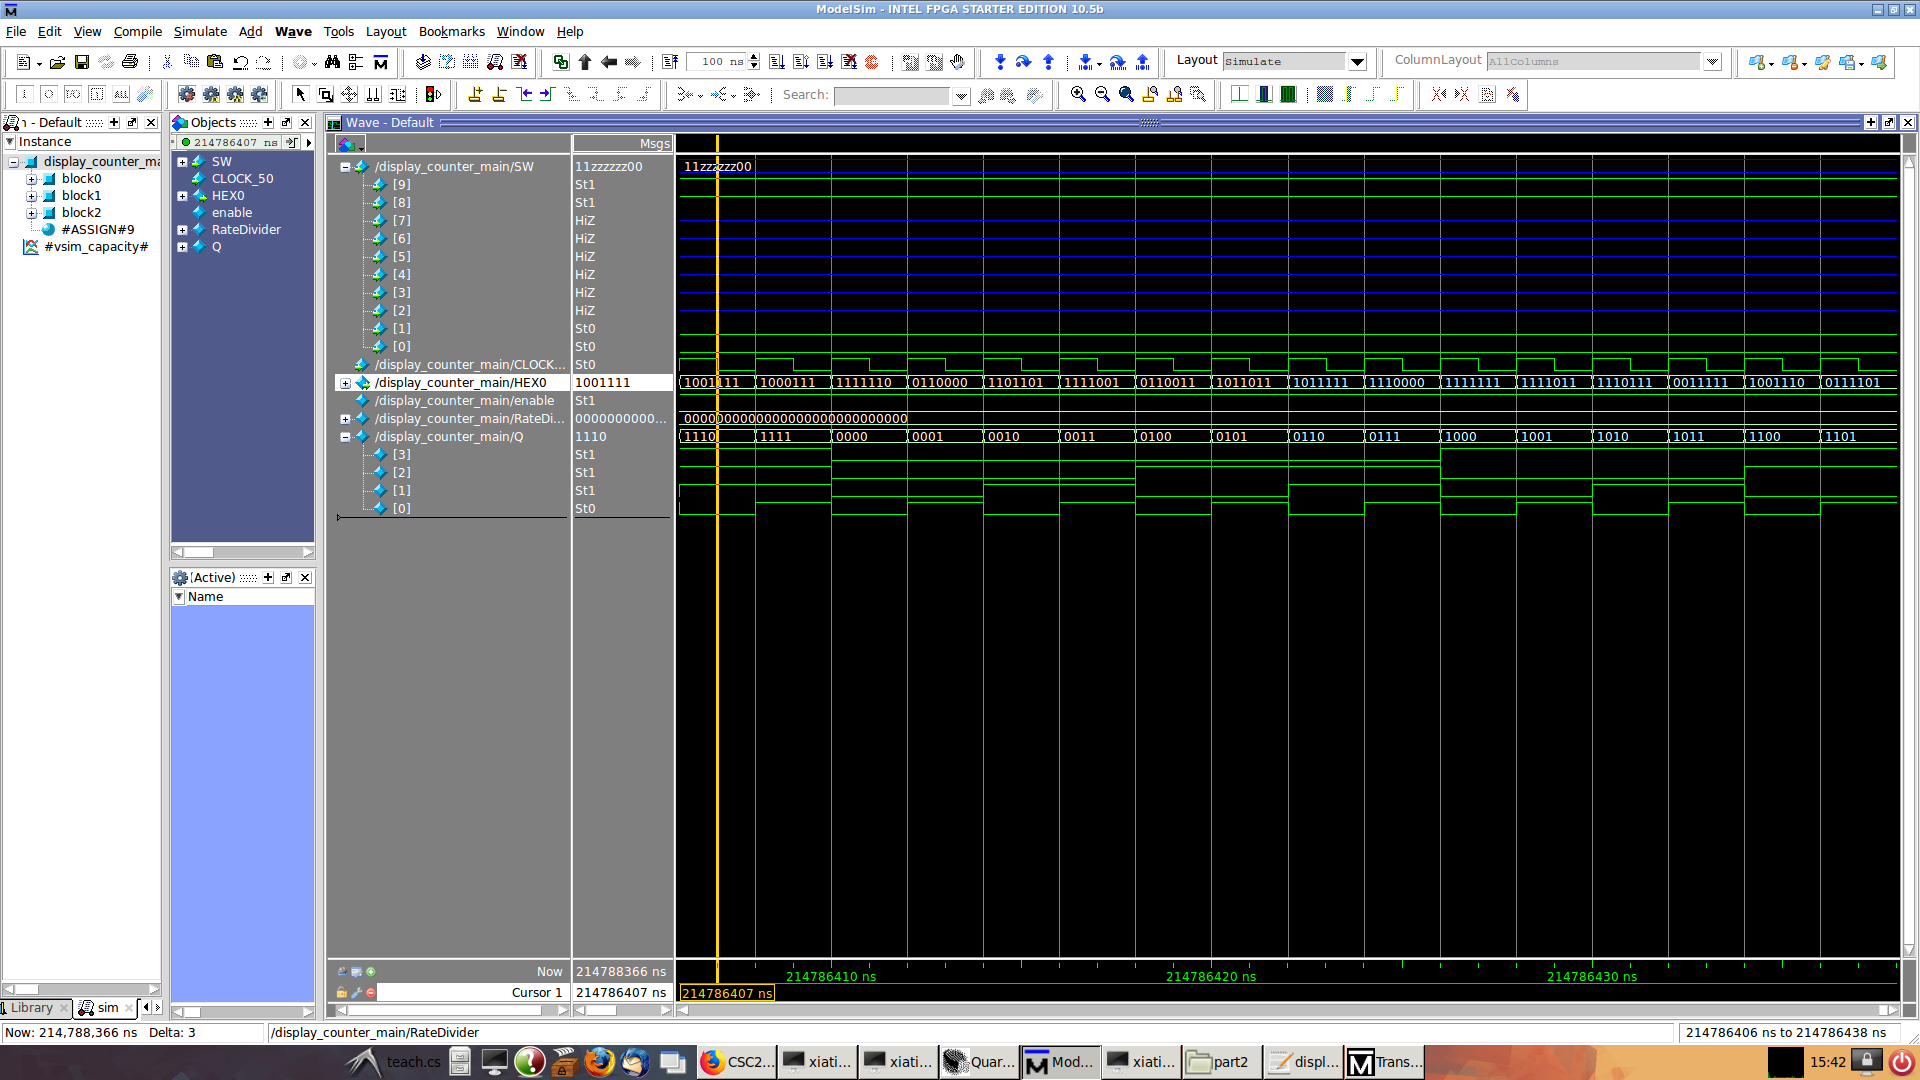
\includegraphics[scale=0.25]{q2_00_slow.png}
\end{center}

\section*{Part 3}
\paragraph{(1)} See the below table, 13 bits length decided by the longest representation (Y) and 0 as seperation.
\begin{center}
    \begin{tabular}{|c|c|c|}
    \hline
    Letter & Morse code & Pattern (len = 13bits) \\ \hline
    S      & ...        & 1010100000000         \\ \hline
    T      & -          & 1110000000000         \\ \hline
    U      & ..-        & 1010111000000         \\ \hline
    V      & ...-       & 1010101110000         \\ \hline
    W      & .--        & 1011101110000         \\ \hline
    X      & -..-       & 1110101011100         \\ \hline
    Y      & -.--       & 1110101110111         \\ \hline
    Z      & --..       & 1110111010100         \\ \hline
    \end{tabular}
\end{center}

\paragraph{(2)} Here is my design schematic
\begin{center}
	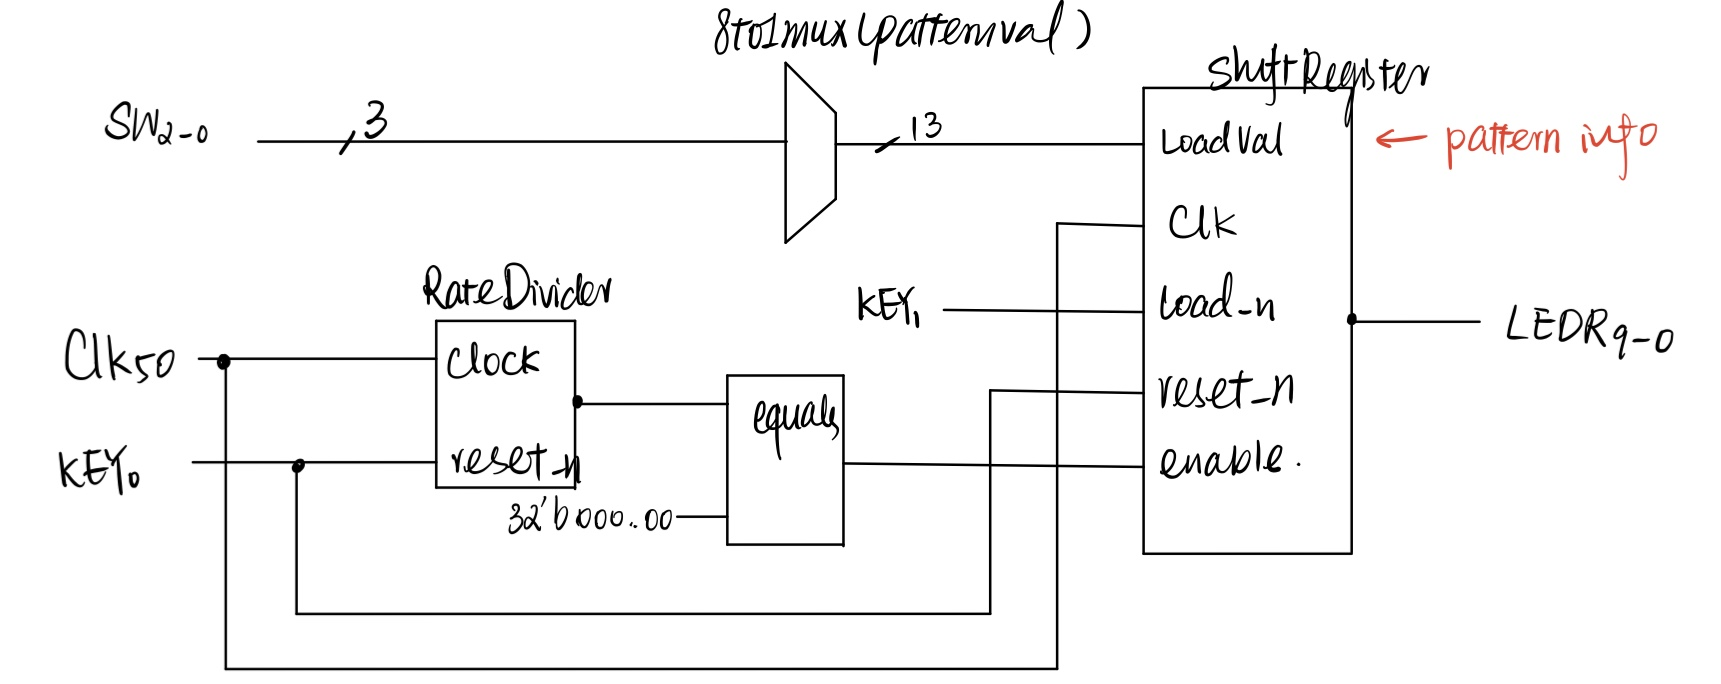
\includegraphics[scale=0.25]{q3_scheme.jpg}
\end{center}
\paragraph{(3)} Here is the verilog code corresponding to the schematic drawn above
\begin{minted}{verilog}
    module morse_encoder_main(KEY, SW, LEDR, CLOCK_50);
    	input [1:0] KEY;
    	input [2:0] SW;
    	input CLOCK_50;
    	output [9:0] LEDR;
    	
    	wire [12:0] shift_register_load;
    	wire [27:0] divider_count;
    	wire enable;
    	assign enable = (divider_count == 0) ? 1 : 0;
    	
    	LUT block0(
    		.c(SW[2:0]),
    		.m(shift_register_load)
    	);
    	
    	rate_divider block1(
    		.clock(CLOCK_50),
    		.reset_n(KEY[0]),
    		.count(divider_count)
    	);
    	
    	shift_register block2(
    		.enable(enable),
    		.LoadVal(shift_register_load),
    		.reset_n(KEY[0]),
    		.Load_n(KEY[1]),
    		.clk(CLOCK_50),
    		.out(LEDR[0])
    	);
    endmodule
    	
    module LUT(c, m);
    	input [2:0] c;
    	output reg [12:0] m; //output's length is 13 bits
    	
    	always @(*)
    	begin
    		case(c[2:0])
    			3'b000: m <= 13'b0000000010101;
    			3'b001: m <= 13'b0000000000111;
    			3'b010: m <= 13'b0000001110101;
    			3'b011: m <= 13'b0000111010101;
    			3'b100: m <= 13'b0000111011101;
    			3'b101: m <= 13'b0011101010111;
    			3'b110: m <= 13'b1110111010111;
    			3'b111: m <= 13'b0010101110111;
    		endcase
    	end
    	
    endmodule
    
    module rate_divider(clock, reset_n, count);
    	input reset_n;
    	input clock;
    	output reg [27:0] count; 
    
    	always @(posedge clock)
    	begin
    		 if (reset_n == 1'b0)
    			  count <= 5 * (10 ** 7) / 2 - 1;
    		 else if (count == 0)
    			  count <= 5 * (10 ** 7) / 2 - 1;
    		 else
    			  count <= count - 1;
    	end
    
    endmodule
    
    module shift_register(enable, LoadVal,  reset_n, Load_n,  clk, out);
    	input enable;
    	input reset_n;
    	wire ShiftRight;
    	input clk;
    	input Load_n;
    	input [12:0] LoadVal; //connected to LUT
    	wire [12:0] Q;
    	output out;
    	assign out = Q[0];
       
    	assign ShiftRight = (enable == 1) ? 1 : 0;
    	
    	ShifterBit sb12(
    		.enable(enable),
    		.load_val(LoadVal[12]),
    		.in(0),
    	   .shift(ShiftRight),
    		.load_n(Load_n),
    		.reset_n(reset_n),
    		.out(Q[12]),
    		.clk(clk)
    	);
    	
    	
    	
    	ShifterBit sb11(
    		.enable(enable),
    		.load_val(LoadVal[11]),
    		.in(Q[12]),
    	   .shift(ShiftRight),
    		.load_n(Load_n),
    		.reset_n(reset_n),
    		.out(Q[11]),
    		.clk(clk)
    	);
    	
    	
    	
    	
    	ShifterBit sb10(
    		.enable(enable),
    		.load_val(LoadVal[10]),
    		.in(Q[11]),
    	   .shift(ShiftRight),
    		.load_n(Load_n),
    		.reset_n(reset_n),
    		.out(Q[10]),
    		.clk(clk)
    	);
    	
    	
    	ShifterBit sb9(
    		.enable(enable),
    		.load_val(LoadVal[9]),
    		.in(Q[10]),
    	   .shift(ShiftRight),
    		.load_n(Load_n),
    		.reset_n(reset_n),
    		.out(Q[9]),
    		.clk(clk)
    	);
    	
    	ShifterBit sb8(
    		.load_val(LoadVal[8]),
    		.in(Q[9]),
    	   .shift(ShiftRight),
    		.load_n(Load_n),
    		.reset_n(reset_n),
    		.out(Q[8]),
    		.clk(clk)
    	);
    	
    	ShifterBit sb7(
    		.enable(enable),
    		.load_val(LoadVal[7]),
    		.in(Q[8]),
    	   .shift(ShiftRight),
    		.load_n(Load_n),
    		.reset_n(reset_n),
    		.out(Q[7]),
    		.clk(clk)
    	);
    	
    	ShifterBit sb6(
    		.enable(enable),
    		.load_val(LoadVal[6]),
    		.in(Q[7]),
    	   .shift(ShiftRight),
    		.load_n(Load_n),
    		.reset_n(reset_n),
    		.out(Q[6]),
    		.clk(clk)
    	);
    
    	ShifterBit sb5(
    		.enable(enable),
    		.load_val(LoadVal[5]),
    		.in(Q[6]),
    	   .shift(ShiftRight),
    		.load_n(Load_n),
    		.reset_n(reset_n),
    		.out(Q[5]),
    		.clk(clk)
    	);
    	
    	ShifterBit sb4(
    		.enable(enable),
    		.load_val(LoadVal[4]),
    		.in(Q[5]),
    	   .shift(ShiftRight),
    		.load_n(Load_n),
    		.reset_n(reset_n),
    		.out(Q[4]),
    		.clk(clk)
    	);
    	
    	
    	ShifterBit sb3(
    		.enable(enable),
    		.load_val(LoadVal[3]),
    		.in(Q[4]),
    	   .shift(ShiftRight),
    		.load_n(Load_n),
    		.reset_n(reset_n),
    		.out(Q[3]),
    		.clk(clk)
    	);
    
    
    
    	ShifterBit sb2(
    		.enable(enable),
    		.load_val(LoadVal[2]),
    		.in(Q[3]),
    	   .shift(ShiftRight),
    		.load_n(Load_n),
    		.reset_n(reset_n),
    		.out(Q[2]),
    		.clk(clk)
    	);
    
    
    	ShifterBit sb1(
    		.enable(enable),
    		.load_val(LoadVal[1]),
    		.in(Q[2]),
    	   .shift(ShiftRight),
    		.load_n(Load_n),
    		.reset_n(reset_n),
    		.out(Q[1]),
    		.clk(clk)
    	);
    
    	
    	ShifterBit sb0(
    		.enable(enable),
    		.load_val(LoadVal[0]),
    		.in(Q[1]),
    	   .shift(ShiftRight),
    		.load_n(Load_n),
    		.reset_n(reset_n),
    		.out(Q[0]),
    		.clk(clk)
    	);
    	
    endmodule
    
    
    module ShifterBit(enable, load_val, in, shift, clk, load_n, reset_n, out);
    	input load_val; // load_val should be 1 bit for every ShifterBit
    	input in; // in is also 1 bit for every ShifterBit.
    	input shift;
    	input load_n;
    	input reset_n;
    	input clk;
    	input enable;
    	output out;
    	wire mux1_to_mux2;
    	wire data_to_dff;
    	
    	
    	mux2to1 mux1 (
    		.x(out),
    		.y(in),
    		.s(shift),
    		.m(mux1_to_mux2)
    	);
    	
    	
    	mux2to1 mux2 (
    		.x(load_val),
    		.y(mux1_to_mux2),
    		.s(load_n),
    		.m(data_to_dff)
    	);
    	
    	d_flip_flop dff (
    		.d(data_to_dff),
    		.q(out),
    		.clock(clk),
    		.reset_n(reset_n),
    		.enable(enable)
    	);
    	
    endmodule
    
    
    module mux2to1(x, y, s, m);
        input x; //selected when s is 0
        input y; //selected when s is 1
        input s; //select signal
        output m; //output
      
        assign m = s & y | ~s & x;
        // OR
        // assign m = s ? y : x;
    
    endmodule
    
    module d_flip_flop(d, clock, q, reset_n, enable);
    	// one-bit d flip-flop.
    	input d;
    	input clock;
    	input reset_n;
    	input enable;
    	output q;
    	reg q;
    	
    	always @(posedge clock, negedge reset_n) // Asynchronous reset from reset_n
    	
    	begin
    		if (reset_n == 1'b0)
    			q <= 0;
    		else
    			q <= d;
    	end
    	
    endmodule
\end{minted}
\paragraph{(4)} ModelSim results\footnote{This was not required in the prelab, but I did it anyways}, resetting. 
\begin{center}
    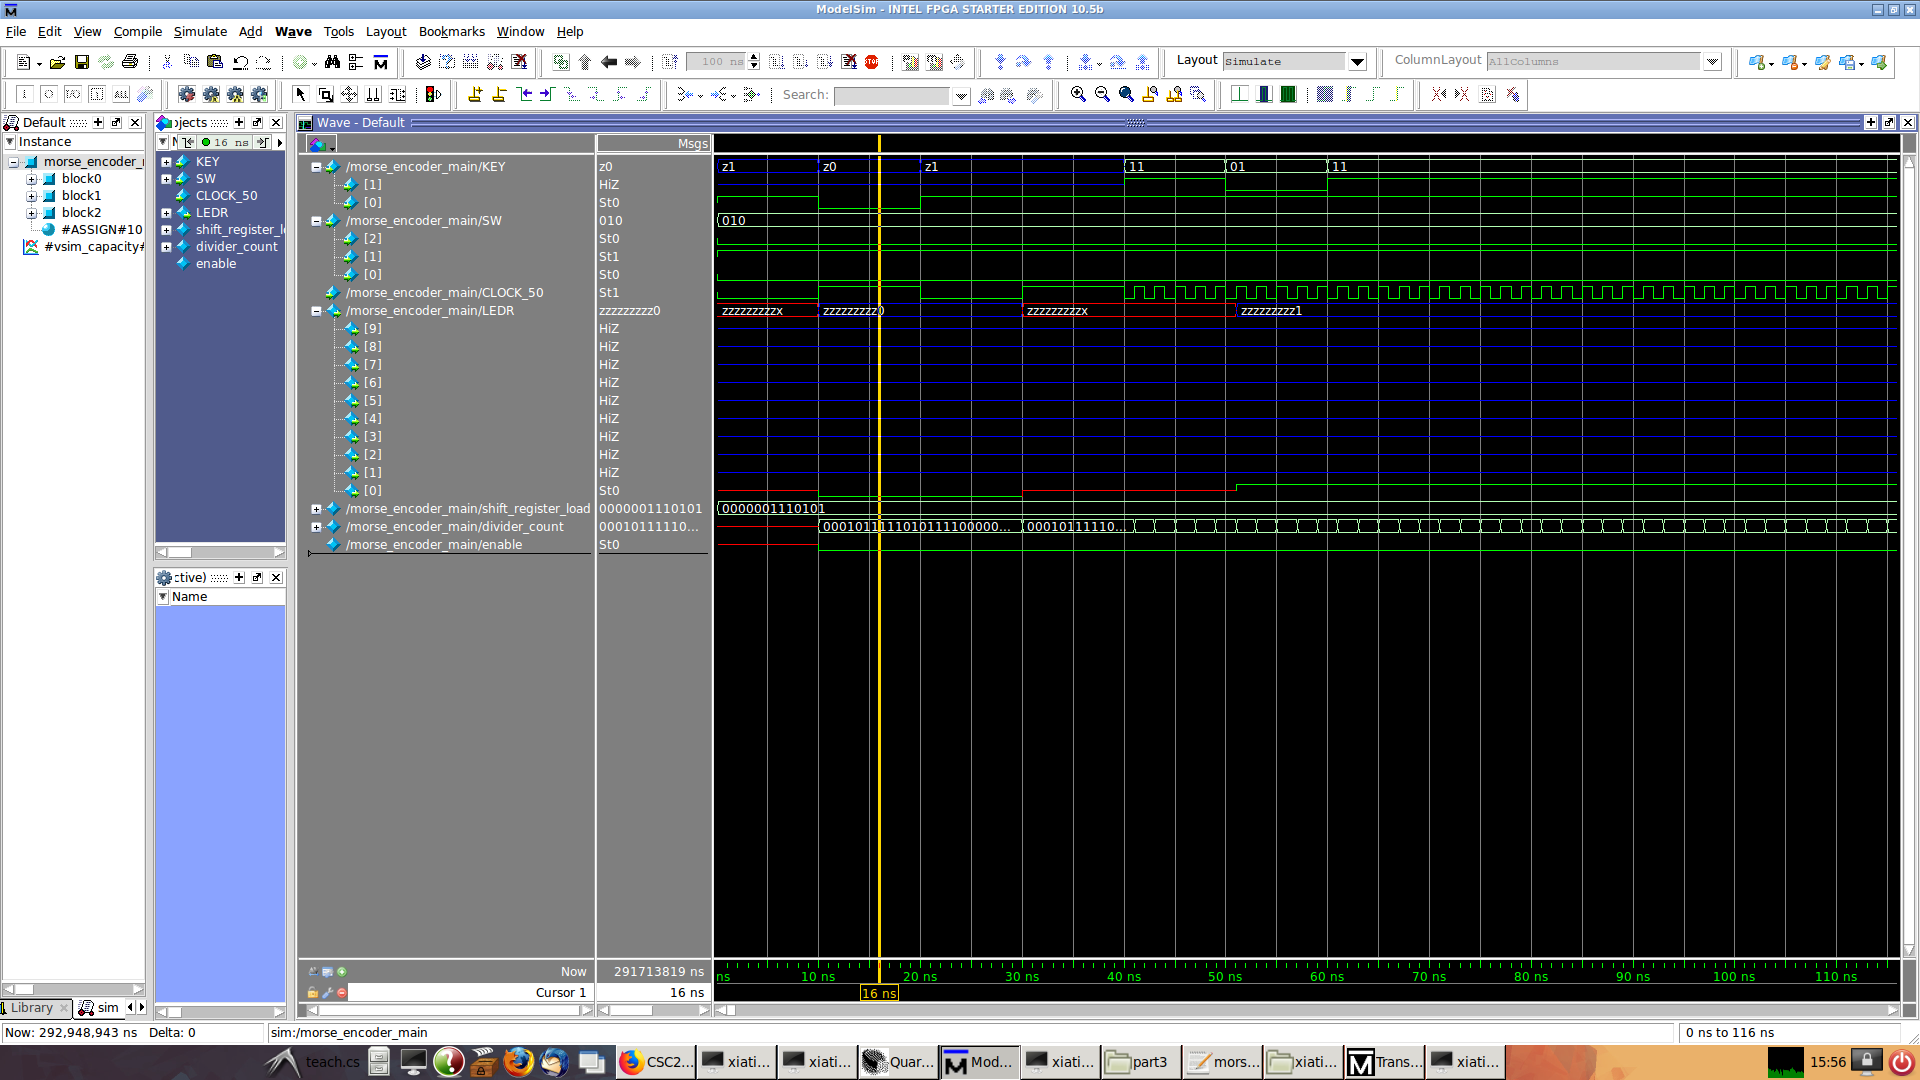
\includegraphics[scale=0.25]{q3_init_reset.png}
\end{center}
The below screen shot is NOT COMPLETE but one can already see the results. The test case that I choose was character U (morse code is dot dot bar, which is 1010111 + zeros).
\begin{center}
    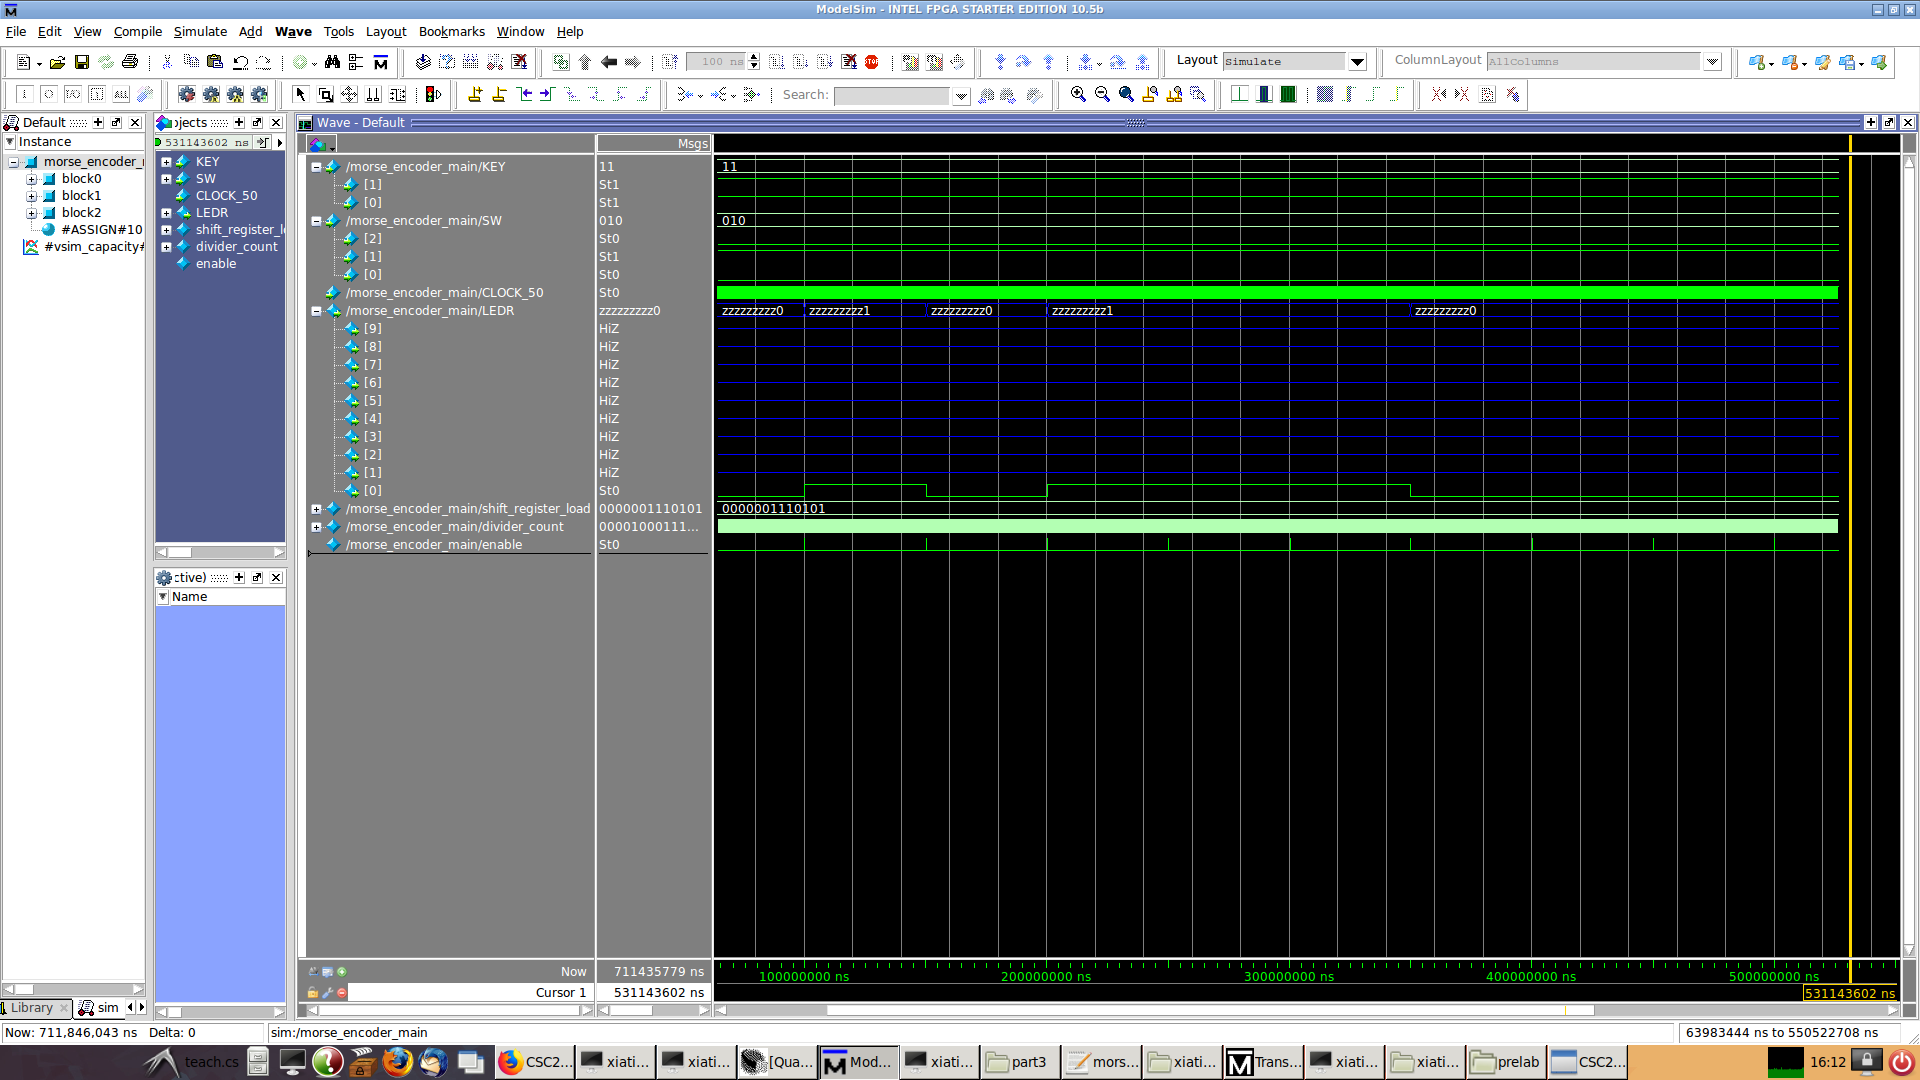
\includegraphics[scale=0.25]{q3_sim_u.png}
\end{center}

\end{document}
